\documentclass[hidelinks,12pt]{article}
\usepackage{hyperref}
\usepackage{enumitem,changepage,lipsum,titlesec}
\usepackage{cite}
\usepackage{comment, xcolor}
\usepackage[pdftex]{graphicx}
  \graphicspath{{images/}, {images/stat/}}
  \DeclareGraphicsExtensions{.pdf,.jpeg,.png, .jpg}
\usepackage[cmex10]{amsmath}
\usepackage{array} 
\usepackage{subfigure} 
\newcommand{\grey}[1]{\textcolor{black!30}{#1}}
\newcommand{\fref}[1]{Figure \ref{#1}}

\oddsidemargin0cm
\topmargin-2cm %I recommend adding these three lines to increase the
\textwidth16.5cm %amount of usable space on the page (and save trees)
\textheight23.5cm

\makeatletter
\renewcommand\paragraph{\@startsection{paragraph}{4}{\z@}%
            {-2.5ex\@plus -1ex \@minus -.25ex}%
            {1.25ex \@plus .25ex}%
            {\normalfont\normalsize\bfseries}}
\makeatother
\setcounter{secnumdepth}{4} % how many sectioning levels to assign numbers to
\setcounter{tocdepth}{4}    % how many sectioning levels to show in ToC


\begin{document}
\title{Dynamic Energy Mapping Project Outline}
\maketitle
\tableofcontents
\newpage
\begin{abstract}
  This document provides an approach of adding the ``time'' dimension
  to an Energy Map. The approach is demonstrated with a model of a
  conceptual urban setting created in CityEngine based on the
  extracted topological and density pattern from an existing urban
  design project. The buildings in the conceptual model is then
  assigned an energy profile of certain DOE Commercial Benchmark
  Building Reference model based on its building type. Hourly energy
  demand profile of heating and cooling end use is then obtained from
  the EnergyPlus simulation of DOE Commercial Benchmark models. The
  energy consumption data is classified into groups with consideration
  of building energy design context and the data distribution
  properties. A corresponding color coded energy profile is then
  generated and imported to CityEngine. 8760 color coded 3D map images
  was then extracted from CityEngine with Python script. A series of
  data reading, plotting, data classification and color-coding
  calculation utilities were implemented. A interactive interface for
  visualizing the images and dynamic data plot with sliders is
  implemented using Python and related packages. The tool is
  anticipated to provide decision support for community energy
  management and planning, demand-side strategy design and district
  system sizing.
  
  The document will also briefly discuss one of the test-bed for data
  classification and visualization.

\end{abstract}
\newpage

\section{General Introduction}
\subsection{Project Overview}
Buildings alone account for 40\% of the total energy usage in the
United States. However the indirect energy impact of the built
environment as a whole was considered, the community design induced
energy and environmental impact could exceed this already high
ratio. The focus of reducing energy usage in the building sector has
once been focused only on the scale of individual buildings and
equipment~\cite{Jaccard19971065}. Community level urban design and the
infrastructure layout can inevitably influence the overall energy
throughput by influencing people's life pattern, energy using behavior
and waste production.

Community Energy Management (CEM) is a combination of community level
design strategies and energy management strategies aiming at providing
quality of life in an urban environment with minimized energy
consumption and environmental impact~\cite{Jaccard19971065}. The
awareness of the importance of the environmental design on energy
performance and quality of life is reflected in design concepts such
as New Urbanism, Smart Growth and Transit-Oriented Growth. These
concepts advocate a compact and pedestrian and bicycle friendly urban
growth that minimizes car usage by creating mixed-used communities,
well-functioned road, complete public transportation system and
diverse housing choices~\cite{smartGrowthWiki}.

The core of the community energy management is to match the demand and
supply as close as possible in terms of energy and
exergy~\cite{Dobbelsteen2013}. CEM reduces energy use impact by 1)
distributed energy generation with sustainable energy source that
close in exergy to the demand side, 2) application of district energy
system that reuses waste heat 3) energy cascading that arranges the
demand side as a chain of decreasing exergy demand so that the entropy
generation is minimized 4) smart grid system that makes electricity
demand and supply match.

Energy Map provides great opportunity to execute the CEM strategies
since it accords with the concept of ``Geo-design'', a
performance-based design method, and makes the energy performance
metrics of community design and management alternatives visible to
planners and policy makers. It facilitates quantitive comparison of
design alternatives and informs better decision making. However the
temporal variation of energy performance metrics is missing from the
majority of current Energy Maps, leading to a simplified picture of
energy impact of design choices and poor decision making such as
excessively over-sized infrastructure systems and loss of energy
recovery and reuse opportunities.

Dynamic Energy Map reveals the temporal variation and better serves
``Geo-design'' approach by revealing the problem of such simplified
pictures of energy supply and demand and support better time-of-use
energy system design, community energy management and policy making.

The current project aims at exploring how a Dynamic Energy Map can
serve as decision support tool for Community Energy Management, more
specifically, to support district energy system design. The focus of
the study is not on exploiting the energy using behavior of a specific
site, but rather a exploration of a generic methodology of Dynamic
Energy Map, thus the map setting is based on a conceptual city model
with a size (68 buildings) comparable to the typical service area of a
district energy system (combined heating and cooling), about 50 to 150
buildings~\cite{IDEA2005}. The Dynamic Energy Map is built upon annual
hourly heating (gas) and cooling energy consumption (electricity) data
from DOE Commercial Benchmark Building simulation. City Engine is used
in 3D urban environment image generation with each building
color-coded according to its hourly energy demand. An interface is
then designed to achieve the ``dynamic'' function with sliders to
navigation through the 8760 hours through a year and present the
energy consumption data in the form of 3D color-coded map and 1D
energy consumption data plot.

\subsection{Objective and Problem Definition}
The objective of this study is to explore the power of Dynamic Energy
Map with a use case scenario of supporting district energy system
design, which is one of the infrastructure side strategy used in
community energy management. Aligned with this major goal, there are
two sub-goals of the project: evaluating some possible approaches to
implement dynamic energy map and presenting one major implementation
approach
\subsection{Outline}

\grey{summary of each section of the report here...}

\subsection{Related Concepts}
Before diving into details about the specific project, it is necessary
to clarify some key concepts including district energy system and
Community Energy Planning, Energy Map and Dynamic Energy Map.

\subsubsection{District Energy System}
A district energy system consists of a power plant, a series of
buildings as terminal energy users and a network of pipelines that
transmit energy from the power plant to end-users. It can supply
heating energy and service hot water to terminal buildings and can
also serve cooling energy with absorption chillers. Commonly used
media for energy transmission include steam, hot water or chilled
water~\cite{baird2014}. A district energy system helps reducing
negative environmental impact by harvesting residual energy in the
form of rejected thermal energy in the process of electricity
generation (CHP based district system) or other industrial
processes. It can adapt to a broader range of fuel choices including
natural gas, oil, coal, waste, and renewable energy sources. This
makes it more flexible and more competitive in the market and
increases the energy system resilience~\cite{IDEA2005}. Other
non-environmental benefits include reducing the space dedicated to
mechanical system and improve building design flexibility, reducing
harmful gas production from stand-alone boiler combustion.  It also
reduces the building initial cost: comparing with a district system
heat exchanger, a stand-alone chiller usually need 30\% to 100\% more
cooling capacity, which means larger system initial
cost~\cite{IDEA2005}.

District systems are most commonly connected to high density urban
environment, university campuses, hospitals and military bases as a
result of their high demand in heating energy or service hot
water~\cite{IDEA2005}. This brings the power generation near to the
power end users, and reduced the transmission loss of both heat and
electricity.

Combined Heat and Power Plant (CHP) is one of the major central plant
used in a district energy system. Traditional electricity generation
central plant has only about 1/3 of the energy turned into electricity
and the remaining 2/3 are rejected as waste heat to the
environment. CHP plant can reduce the amount of reject heat to 20\%
and the recovered heat are supplied to surrounding buildings for space
heating or cooling~\cite{IDEA2005}.CHP plant can also be equipped with
back-up boilers, electric boilers, and thermal storage that help shift
the peak thermal and electric demand and production and provide
reliable supply of thermal energy and electricity~\cite{IDEA2012}.

One famous example of CHP based district system is the Sheffield
District Energy Network in UK. The Sheffield District Energy Network
is a system that started to provides the local buildings with heat and
electricity since 1988. It is owned by the City Council and is
operated by Veolia Environmental Service. The system consists of an
Energy Recovery Facility (ERF) located in the center of Sheffield, a
series of wires and pipes that transfer electricity and heat in the
form of hot water to local buildings and the terminal heat exchanger
installed in the local buildings receiving the heat from the
network. Electricity generation is based on waste combustion
process. Local garbage is collected each day and is transmitted to the
tipping hall of the ERF via a short distance with low CO$_2$ emission
vehicles. The collected garbage goes through a combustion process in
the boiler and produces 400 $^{\circ}$C high pressure steam and flue
gas. The latter is treated and emitted to the atmosphere with 10\% to
60\% less pollutant below required level. The former enter the turbo
generator to generate electricity. 19 MW of electricity is generated
and is supplied to 22600 local homes. After going through the
electricity generator, the 400$^\circ$C steam is de-pressured. It
enters a heat exchanger and transfers the heat to hot water. The hot
water is then sent to the local buildings and provides these buildings
with space heating~\cite{veolia2014}. 
\begin{figure}[htbp]
  \centering
  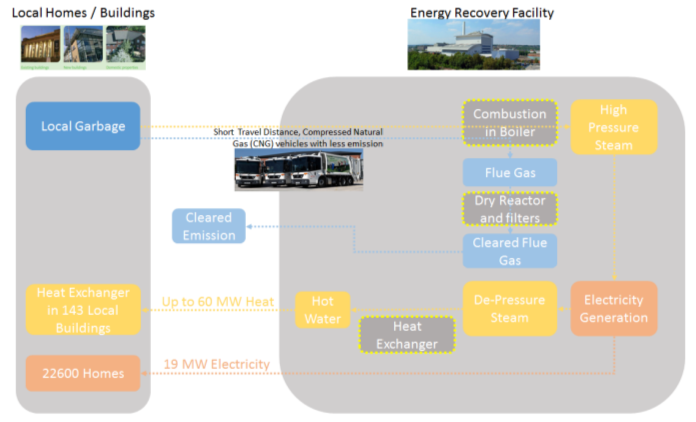
\includegraphics[width=0.7\linewidth]{sheffield.png}
  \caption{Sheffield District System}
  \label{fig:sheffield}
\end{figure}

Energy Map helps the assessment of whether a building is suitable to
be connected to the district system according to its heat demand
density. A common boundary is 0.93$kWh/ft^2$ (IEA) or 26.5 MMBtu per
square mile~\cite{IDEA2012}.

Energy Map was used in analyzing the potential extension of the
Sheffield District System by mapping the buildings or regions that
have high head demand and potential heat suppliers that adds
additional heat supply capacity to the existing
system~\cite{Finney2012165}, for more detailed information please
refer to section \ref{infra}.

\subsubsection{Definition of Energy Map}
\paragraph{Energy Thematic Map}
In a restricted sense, Energy Map is an instance of a thematic map
that depicts energy information. It is an abstract representation of
some energy feature in an urban environment. It is useful in providing
energy related qualitative or quantitative insight. 

The energy topics depicted in an Energy Map can be classified into
four major categories: energy supply, energy demand, energy related
building design / urban planning, and energy related environmental
impact. One common sub-category of the supply side topics concerns the
locations and evolving process of energy infrastructures such as power
plants, energy transmission pipelines, energy refining facilities and
market hubs. EIA state energy profile map~\cite{EIAProfile2015},
U.S. natural gas pipeline map~\cite{EIAGaspipe} are under this
sub-category. Other supply side topics include total energy production
~\cite{DOEEnergyProduct}; total energy source production like global
coal production map~\cite{EIACoalProduct}; sustainable energy
potential map of wind, solar, biomass, geothermal energy
potential~\cite{NRELMap2015} and hidropower
potential~\cite{DOEHydro}. Common demand side topics include: energy
demand for one or more enduses ~\cite{heatMap2012}, energy source
demand like coal demand ~\cite{EIACoalDemand} and energy cost
~\cite{DOEEnergyCost}. The design side topics concerns building
physical conditions like Calgory Heat Map ~\cite{Hay2011}, design
policy information like climate zone map~\cite{IECCClimate} and energy
code adoption map~\cite{CodeAdopt}. The energy behavior environmental
impact map include both the impact of building or energy
infrastructure to environment and the environment change to buildings
or infrastructures. The carbon emission map as ~\cite{CO2Atlas} is an
instance of the former and the ``Energy Sector's Vulnerabilities to
Climatic Conditions'' Map is an example of the
latter~\cite{DOEVulner}.

It is necessary to mention some unfortunate terminology overloading
involved in the topic of Energy Map. The term ``Heat Map'' used in
this discussion refers to the Energy Map with building heating energy
as its theme, not to be mis-interpreted as the color-coded
representation of matrix values as in this
definition~\cite{HeatmapWiki}.

The history of thematic map dates back to early 17th century, and from
then on maps can present spatial patterns of some feature in addition
to merely recording locations of geographic
features~\cite{ThematicMap}. Over a century later, spatial analysis
emerges and map starts to assisting Geo-data analysis. Finally after
the born of modern computer and the development of database, map
becomes a more powerful information system that undertakes more
complicated tasks including data aggregation, managing, query and
presentation. This gives Energy Map a much broader meaning.

\paragraph{Geo-database of Building Energy}
In a broader sense, Energy Map is a hibernation of two types of
databases: building energy database, a subset of the BIM (Building
Information Model), and Geographical Information System (GIS). The
basic functions of an Energy Map includes 1) storing energy data in an
organized fashion, that facilitate easy analysis and query of energy
data and 2) provide reports in the form of graphs, tables, animations
etc that conveys numerical information in a way that best support
pattern recognition and decision making. 

This definition can be considered as a super set of the thematic map
definition, so the energy topics inherits those representable in the
thematic energy map. Some examples of the Energy Maps under this
``database'' definition include: National Heat Map that records and
presents heat demand density of buildings and building sectors,
Renewable Energy Potential Map that uses GIS tool in renewable and
residual energy potential assessment~\cite{Voivontas1998333}, a site
selection model that evaluates different choices of power plant
location~\cite{Yeo201499}, and ``Heat maps'' with information of heat
sources and sinks that supports district system expansion
design~\cite{Finney2012165}.

\paragraph{Coupled Geo-database and Energy Simulation Platform}
``Geo-design is a design and planning method which tightly couples the
creation of design proposals with impact simulations informed by
geographic contexts''~\cite{Flaxman2010}. It is a performance based
approach in urban and environmental planning. Traditionally, each
performance metric is represented with a choropleth map layer. By
stacking these layers together, the performance metrics are aggregated
for each location on the map and a judgement of design alternatives
are formed based on the aggregated performance
metrics~\cite{CPcp66-goodchild}. However, some of the performance
metrics require complicated calculation or simulation, especially
those with temporal variations. Hence the new development of Energy
Map will not only record data but also ``produces data'' by providing
smooth connections to urban level energy simulation tools that
calculates energy performance metrics of different design alternatives
on the fly. This enhanced Energy Map may effectively automates
the Geo-design work flow.

\subsubsection{Definition of Dynamic Energy Map}
Within the current context, ``dynamic'' refers to changing over time,
hence Dynamic Energy Map is an Energy Map equipped with temporal
information. Sometimes this type of map is referred to as
``spacetime'' map~\cite{Brownrigg2005}. As a result of the ``dynamic''
property, one assumption about Dynamic Energy Map is that at least one
of the energy related variables depicted in the map should change over
time. Due to the fact that there are three versions of definitions for
Energy Map, there are also three versions of corresponding Dynamic
Energy Map.

\paragraph{Thematic Map Time Series}
In a restricted sense, where an Energy Map is defined as a thematic
map focusing on energy topics, Dynamic Energy Map is just a series of
maps, each of which is a thematic Energy Map representing the status
of energy information happened at a certain time spot. Also with the
convention that thematic maps are ordered in increasing time order.
The purpose of such a Dynamic Energy Map is to facilitate the
comparison of thematic maps at different time steps. Baring this in
mind, it makes more sense to apply a universal map symbol and
breakpoints to the sequence of thematic maps in this version of
Dynamic Energy Map.

\paragraph{Spatial-Temporal Energy-Geo-database}
In a broader sense, where Energy Map is defined as
energy-Geo-database, Dynamic Energy Map is an energy-Geo-database with
``time'' being one of its data entries. One major purpose of Dynamic
Energy Map under this definition is to enable search, filter and query
of the energy data by ``time'' field, thus presumably, time should act
as one of the indexes in the database that facilitates faster search
and query of the time data.  The second task of Dynamic Energy Map is
to provide more powerful reporting tools than normal Energy Maps that
accounts for the difficulty and complexity of spatial-temporal data
visualization aiming at better conveying the dynamic spatial
pattern.

\paragraph{Performance Based Geo-design Support Platform}
When Dynamic Energy Map becomes a platform coupled with Energy
Simulation tools, design alternatives would be evaluated and compared
at each given time spot or time window according to the design
context. This enables more detailed energy analysis.

\subsubsection{Definition of Dynamic Energy Map for Supporting
  District System Design}
District system supply thermal energy to the surrounding community,
thus the community heating or cooling demand decide the size of a
district system. Therefore heating demand and cooling demand are
selected as the major variables in the study. We define ``Local''
Dynamic Energy Map for community level design support as:
\begin{itemize}
\item A database holding 8760-hour meta data of energy demand of
  buildings in a moderate sized community served by a district
  system~\cite{baird2014}.
\item An interface that has multi-dimensional graphical display of the
  meta data.
\end{itemize}

The data display should include 1D data plot, 2D or 3D map and 4D
temporal-spatial navigation:
\begin{itemize}
\item 1D: data plot for providing quantitative information of energy
  demand or supply

  The Local Dynamic Energy Map displays the aggregated hourly energy
  demand of the whole community and major building sectors throughout
  the year. It enables comparison of different urban design
  alternatives in terms of total demand and demand variation. This
  information supports district system planning by arranging land use
  design to minimize total load variation.

\item 2D or 3D: graphical display of spatial relationship of energy
  data

  The Local Dynamic Energy Map applies a graduated symbol or color to
  buildings in the community to provide the intuition of the building
  energy demand changing within a community. It helps identify the
  rank of energy demand in a community and provides a guidance in
  energy cascading design.
    
  For univariant map scenario, we suggest the variant size symbol
  according to the study ~\cite{Garlandini2009,
    doi:10.1559/1523040639298}. For bivariate map
  scenario~\cite{bimapWiki} in 3D map design, we suggest the bivariate
  choropleth map representation. For detailed explanation of this
  design choice please refer to section \ref{mapDesign}.

\item 1D + 2D or 3D: interactive graphical display of spatial-temporal
  pattern of energy data.
  
  The Local Dynamic Energy Map compares energy demand of different
  time of year by providing a easy navigation with a time
  slider. Energy demand of each time spot is expressed with 2D or 3D
  map and 1D data plot.
\end{itemize}

\subsection{Why ``time'' dimension is important for an Energy Map}
\subsubsection{Strong Temporal Variation of Energy Demand}
Building energy demand is strongly dependent on weather condition,
building type, size, building physical design, building mechanical
system and appliance quality and building operation schedules.  The
aggregation of all parameters results in a great variation in the
range and extreme value of energy consumption. Weather condition have
strong seasonal pattern and day-night pattern. This type of variation
takes the form of a global influence on building heating or cooling
load. Building operation schedules vary greatly from building to
building as a result of difference in building type and occupant
behavior. Different operation schedules indicates the arrival of peak
demand within a mixed-use urban environment are not
simultaneous. Difference in building type also suggest difference in
indoor environment requirement such as ventilation rate, lighting
intensity etc., indicating a dramatic variation in energy consumption
data distribution among buildings in the community.

\subsubsection{More Detailed Description of Energy Behavior Supports
  Better Design}
A simple annual or monthly average cannot effectly represent the real
energy consumption behavior of an individual building and the whole
urban environment. In order to present this complicated behavior of
time-dependent energy demand, the time dimension is necessary.

For example, hospitals are usually constant heat consumers with very
stable heat demand throughout a year, while a performance center is,
on the other hand, an occasional huge heat consumer with very high
peak demand occuring occasionally at event time and with almost zero
demand in the remaining time. It is reasonable to apply different
energy planning strategy for building groups involving one of these
two types of buildings. However, if time dimension is not included,
one has to choose some form of aggregate description of the energy
consumption, be it average, maximum, minimum or annual total. For most
cases, annual total demand is used for representing a building's
energy demand. With this approach, the different energy usage pattern
of a hospital and a performance center is not differentiable, which
results in a simplified energy plan decision.

\subsubsection{Aggregation of Peak Value Becomes Tricky for Data with Time Variation}
Dynamic Energy Map supports district energy system design by 1)
revealing the non-coincident peak demand of heat or cool 2)
providing the aggregated demand supporting better decision making.

Obvious mathematical concepts sometimes become more obscure when it
comes to real life problems. It is well understood that linearity
holds for expectation not max, i.e. the sum of max values of each
distribution does not equal to the maximum of the sum of values in
each distribution. However this mistake is not rare in the sizing of a
district system. One common approach of sizing a district system is to
add up the capacities of each terminal devices. However, each
individual device is sized to meet its peak demand. Since the peak
demand of individual buildings do not occur at the same time, the end
result of summing up the max demand at each end point exceeds the
actual total demand peak of the community, hence with this approach,
the whole district system becomes excessively over-sized, which reduces
the whole system efficiency. Dynamic Energy Map can reveal the problem
of such approaches by directly providing the aggregated demand and the
demand for single buildings or building sectors side by side,
eliminating the misunderstanding of the aggregated demand and
providing the actual data for system sizing.

\begin{comment}
\subsubsection{Temporal Variation in Energy Generation, Storage
    Devices, Price Variation}
The commonly used renewable energy source includes: solar, wind,
geothermal, hydropower and biomass. Among these sources, solar energy
have strong temporal fluctuation as a result of the temporal variation
of solar radiation between different hours of a year and the time of
year~\cite{EIARenewable2015}. 
\end{comment}

\subsubsection{Close Match of Supply Side to Demand Side Improves
  Community Scale Energy Performance}
As a result of the finiteness of fossil fuels, the using of renewable
energy begins to come into play. In 2013, renewable energy account for
9\% of the primary energy source of residential and commercial
buildings ~\cite{EIAPrimary2013}. Electricity generated from
sustainable sources normally do not have much storage capacity, hence
in order to meet the energy demand with renewable electricity, a
better understanding of the spatial-temporal pattern of energy demand
is important~\cite{Mikkola2014256}.

Demand-driven energy supply is necessary to reduce energy waste and
achieve better total community energy performance. Dobbelsteen et al.\
pointed out that the ``exergetic challenge'' for urban energy supply
is that the building operation requires only low or medium grade
energy, but the supply side is usually with high energy density source
as fossil fuel. In facing of this challenge, renewable energy and
``residual'' energy are in place to ``fill the gap'', providing energy
supply with various energy density, facilitating the cascading
strategy\cite{Dobbelsteen2013}.

In order to match the supply side to the complicated behavior of the
demand side in both energy quantity and quality, understanding the
spatial-temporal pattern of the energy demand in the early design and
planning stage is important.

\paragraph{District System Design}
The time dimension is important to district system design because it
reveals the temporal complexity of the community energy supply and
demand. The ability to describe the energy using behavior with more
details then a mere max, min and average and to classify building
energy demand into more detailed behavior prototypes is the first step
to energy oriented land use plan, demand side energy management and
energy cascading design. This more accurate picture also act as the
basis of further design of energy supply and infrastructure system.

With Dynamic Energy Map, one can classify energy sources and sinks
into more specified categories and design for more specific
combinations of sources and sinks. One can also identify energy
sources and sinks that dynamically changes over time. The
temporal-spatial energy supply and demand information can be helpful
in the following cases:

\begin{itemize}
\item Demonstrating the increased efficiency of district system
  
  Comparing with district system, a single building stand-alone
  equipment are sized according to its peak load, since peak does not
  occur very often for most of the cases, the stand-alone system is
  running on its less efficient power output for the majority of the
  time, hence is less efficient. district system on the other hand, in
  a mixed used community has much stabler aggregated load and can run
  on its optimal output power for longer time than stand-alone system,
  hence is more efficient. This fact can be demonstrated by dynamic
  energy map by comparing the energy throughput of the two cases
  considering the system efficiency.

\item Enable the design of local load balancing

  Large public facilities like stadiums or performance centers
  normally have mechanical systems with large capacity to meet its
  peak demand but the large capacity might only be used under
  occasional event. Dynamic Energy Map helps identify such
  occasional heavy energy consumers and helps optimize landuse
  planing by arranging the right amount of surrounding consumers and
  optimize the local system design by redirect the energy capacity of
  the ocational heavy consumer to surrounding
  buildings~\cite{IDEA2012}
  
  Groups can connect to a shared boiler or chiller, which is then
  connected to the district network. Buildings with different energy
  using profile can make the aggregated load of the group be smoother
  than single building. Such a building group can be served by a lead
  boiler and a backup boiler with the lead boiler constantly running
  on its optimal efficiency and the backup boiler occasionally for
  meeting the peak load~\cite{IDEA2012}. Dynamic Energy Map can
  identify such building groups that has the opportunity to

\item Support the design of connections to district network

  Dynamic Energy Map can identify buildings with consistent high heat
  demand, i.e anchor load building~\cite{IDEA2012} and buildings with
  occasional high heat demand or consistent low heat demand. By
  identify these two types of buildings, urban planners could connect
  the former to the district system and the latter could be connected
  to the former with ambient water loop so that the latter could
  ``borrow'' heat from the former and reduces the community energy
  throughput.

\item Help design of local energy storage devices

  Energy storage devices can shift the peak supply to meet peak
  demand, and it also made the community energy flow more
  complicated. Accurate information of the surplus and deficiency over
  time helps design the storage capacity for single building, building
  group and the whole community central plant.

\item Convey the energy benefit of mixed-land use.

  In a mixed used urban environment, with a mixture of energy demand
  profile, the central plant could potentially operate at optimal
  output level over a longer time period than the single land use
  case~\cite{IDEA2005}. With a Local Dynamic Energy Map, one could
  compare the total energy demand and the demand variation directly
  between the mixed land use case and the single land use case. The
  benefit of community level load balancing could be visible to the
  policy makers and planners to inform better land use design.
  
\end{itemize}

\newpage
\section{Related Works}
\subsection{Static Energy Map}
The majority of existing Energy Map instances are static maps with no
time information. As is mentioned in the thematic map definition, the
major application of Energy Maps include energy supply, energy demand,
building or infrastructure design resulted energy impact and
environmental impact. The sub-section will present some more detailed
examples in each use cases.

\subsubsection{Supply}
\paragraph{Assessing Renewable Energy Potential}
In order to reduce environmental impact, increase resilience of local
energy supply and match energy intensity of supply and demand in urban
environment, renewable energy source of wind, solar, geothermal,
biomass and hydropower becomes an increasingly important energy
source. Comparing with fossil fuel, the energy production with
renewable energy has strong correlations to Geo-locations, thus the
energy map of renewable energy availability and demand can support
energy planning that aims at improve urban scale energy
performance~\cite{Ramachandra20071460}.

Some study focuses only on one type of renewable energy source.

Voivontas et al. developed a decision support tool using GIS for
accessing the wind energy potential in four aspects:the theoretical
potential in terms of wind speed, availability potential in terms of
land use regulations and technological potential in terms of energy
production features of wind turbine and economical potential in terms
of IRR. 

``NYC City Solar Map'' presents solar energy potential for
buildings across the New York city. The map presents solar energy
generation curve, estimated solar system installation area, financial
incentive and payback~\cite{NYCSolarMap}

Other efforts tackles multiple renewable energy sources:

Ramachandra and Shruthi produced a series of district level renewable
energy theoretical potential maps of solar, wind, hydroenergy and
biomass in Karnataka State, India. The potential is estimated based on
data of global solar radiation, wind speed, hydropower plant capacity,
and plantation and livestock information. GIS is used in aggregating
energy potential data to each district. Each type of renewable energy
source is presented as a single variable thematic energy map.

\subsubsection{Demand and Infrastructure}
\paragraph{Analysis or design support of existing energy
  infrastructures}\label{infra}
Finney et al.\ studied the potential expansion opportunities for the
Sheffield district energy network by producing a heat mapping that 1)
depictes heat sources and sinks, including existing ones and emerging
ones 2) identify ``heat zones'' by connecting sources and sinks. The
``heat zone'' is then filtered with concerns of economic feasibility
and environmental impact. The network extension is then designed
based on the remaining ``heat zones''. Heat demand is assessed with
population density for residential buildings and is represented on the
map as polygon features with graduated color. Heat demand for
non-residential buildings are assessed with gas consumption and is
mapped as point features with graduated size. Heat sources are
identified with the criteria ``producing recoverable, low-grade
'waste' heat''~\cite{Finney2012165}. They are mapped as point features
including steelworks, combined heat and power (CHP) plants, and
biomass power stations. The ``heat zone'' is identified based on
abundance of sources or sinks.

National Heat Map is a ``publicly accessible high resolution
web-based'' heating energy interactive map, developed by the
Department of Energy and Climate Change (DECC) in UK. It aimed at
``support planning and deployment of local low-carbon energy projects
in England''~\cite{heatMap2015}. Heating demand density ($kWh/m^2$) of
four major building sectors: public buildings, commercial buildings,
industry buildings and residential buildings, together with the total
demand is plotted on the map as 2D raster feature with a color scheme
from blue to red, with blue for low heating demand and red for high
heating demand. Heat source of CHP stations and ``Thermal Power
Stations'' ~\cite{heatMap2012} are plotted as point features in the
map. Address level heat demand data in csv format is also available
for local authorities~\cite{heatMapLocal2012}. 

The ``Water Source Heat Map'' is an added layer group to the existing
National Heat Map with information about the the heat potential of the
4041 waterways in England. Heat potential of waterways are represented
in temperature, surface area, flow rate and heat capacity ($kJ/m^3$
for coastal and estuary, $kW$ for canal, river and settlement). It
aims at supporting the plan of water-based thermal system as
water-based heat pump~\cite{waterHeatMap}. The map revealed the large
thermal capacity of water bodies that could serve over one million
buildings~\cite{waterHeatMap}.

\paragraph{Energy consumption prediction model}
Kolter and Ferreira presented a modeling method to predict building
energy end use in Cambridge, MA. They also developed a user
application, ``Energy View'' with two target user groups: general
public and local authorities. The model can be used by local
authorities to identify energy usage outliers and by general public to
compare their monthly energy consumption with predicted baseline
consumption.

\paragraph{Smart Management of Urban Energy System}
Energy Map also helps smart management of energy system in a large
urban scale. ``Smart Urban Services for Higher Energy Efficiency''
(SUNSHINE) project is a European Co-Founded project launched in
2013. It is accessible through web page and smart phone or tablet
application. It aims at developing a platform capable of 1) assessing
building energy consumption behavior and create a 2D and 3D energy
map, ``ecomap'' accordingly 2) providing automatic alerts regarding
optimized usage of heating/cooling system 3) remote control of public
building lighting systems~\cite{SUNSHINE2015}. The target users of the
application include facility managers, policy makers, citizens and
energy service companies. Function 1) is anticipated to help energy
company and facility managers to identify energy consuming outliers,
provide information for building pre-certification. Function 2) aims
at providing more accurate baseline consumption data using weather and
meter data. Function 3) allows better management of public lighting
system based on illuminance requirements and weather conditions.

\subsubsection{Combined Supply, Demand and Infrastructure}
Dobbelsteen et al. described a framework of energy potential mapping
that depicts information of energy supply, demand and infrastructure.
Comparing with the previous examples, that 1) in addition to renewable
energy source, it also considered residual energy as energy sources
and 2) aggregated multiple types of energy potentials in a single map
with the unit of GJ or GJ/ha~\cite{Dobbelsteen2013}. The energy
potential of sources are estimated by theoretical potential multiplied
by a serious of ``limiting factors''. The energy demand includes
buildings and transportation. The authors also suggest to map energy
storage on the map. A case study of ``HEAT Mapping'' is presented with
aggregated supply and demand presented in a single 3D Heat Map. The
absolute quantity of each type of demand and supply of a certain
region is represented with extruded height in the 3D map. Demand is
represented with a transparent 3D feature, each supply source is
represented with solid 3D feature in a different color. The
aggregation of information is valuable in answering the question of
whether the supply meets the demand, the representation becomes too
complicated~\cite{Dobbelsteen2013}.

\subsubsection{Reflections}\label{Reflection}
The existing mapping approaches had their main effort in the data
calculation and aggregation, however the resulted visual
representation is questionable for most instances. One common issue is
too much distraction from unthoughtful map symbol design. For
static maps, a poorly designed visual representation might still be
tolerable, but for Dynamic Energy Map with an additional time
dimension, each additional bit of distraction will prevent the
necessary information from getting through. Hence the authors think it
is necessary to discuss the map design aspect, and look for examples
of best practices. This is done in section 3.2.3.

\subsection{Dynamic Map}
The aim of this section is to explore how the time dimension can be
represented in a map.
\subsubsection{Energy Dynamic Map}
Current Dynamic Energy Map instances are mainly 2D animated maps with
large time steps, in large spatial scale and low resolution (state
level), and very few number of frames. These instances include: State
wind power capacity map that depicts the wind industry growth at state
level from 2000 to 2050~\cite{DOEWind}, wind farm development map that
shows the wind farm location and capacity development from 1975 to
2013~\cite{DOEWindFarm}, solar plant development map that shows the
solar plant location and capacity development from 1975 to
2013~\cite{DOESolarPlant}, US Energy Production Map that shows
state wise energy production from 1993 to 2012~\cite{DOEEnergyProduct},
$CO_2$ emission map presenting world-wide carbon emissions from 1980 to
2014~\cite{CO2Atlas}

One instance of the high resolution energy demand dynamic map was
found in the project ``Energy Mapping to Identify Opportunities for
Future Networks''~\cite{Diaz2013}. The aim of the project is to
``analyze the spatial and temporal distribution of energy
consumption'' and support decision making and design of energy network
development. Energy data was retrieved from both metered data and HEM
simulation. Energy Demand Maps of three different resolutions were
created: campus level, community level and city level. For campus and
community level maps, monthly heating demand density dynamic map and
monthly electricity demand density dynamic maps are created with
($kWh/m^2$) as the unit. The energy demand is represented in a scale
from blue to red, the same as the approach of the National Heat
Map. The time dimension is added in the form of a non-interactive 2D
animation . The problem for this animation is the lack of temporal and
spatial legend and its non-interactive nature. Also the heating and
electricity demand is represented separately, making the pairwise
comparison of these two variables difficult.

\subsubsection{History and Archaeology Instances of Dynamic Maps}
Although based on current knowledge of the authors, Energy Maps
equipped with the time dimension is still rare, but there already
exists many instances of dynamic interactive map in History and
Archaeology practices. Pittsburgh Historic Map displays the urban
environment layout of the City of Pittsburgh from 1835 to 2015 using a
combination of historic maps and Google map as the base map. It allows
users to navigate through the times with a time slider. It also
contains point features of historic buildings\cite{EsriHistory2015};
Europe History Interactive Map that demonstrate the changes of
political boundary with historic information associated to each
political entity~\cite{Worldology2009}. User can navigate through
different historic period by forward and backward arrows and by
clicking on specific entries to that period.

\subsubsection{Works on Map Design}\label{mapDesign}
\paragraph{Symbol Chosen}
Dong et al.\ assessed the effectiveness of symbol design and frame
rate on the effectiveness on dynamic map display with two metrics:
deviation and response time. They discovered the change of symbol size
is more effective than color under the same frame rate. They also
identified the optimal class numbers for graduated size symbol (15)
and graduated color symbol (10) on 1024x768 display. The optimal frame
rate identified in the study is 3 for color symbol maps and 6 for size
symbol maps. They also suggest to reduce class number and frame rate
if the display size is smaller than
1024x768~\cite{doi:10.1559/1523040639298}.

\paragraph{Bivariate Map Design} \label{bivariate}
In order to represent heating demand and cooling demand are on the
same map together, we encounter a common map design problem: bivariate
map design problem. Elmer presented eight possible types of
representation for bivariate maps: ``shaded cartographer, rectangle map,
bar chart, value by alpha, choropleth with graduated symbol, bivariate
choropleth, spoke glyph and shaded texture''~\cite{Elmer2012}. In our
current case of 3D representation, to incorporate the map symbol to
the 3D model, the representation with dimensional changes are not
suitable since they will distort the actual building geometry which
makes the urban environment un-realistic. The only choices are the
ones that only involves color or texture, i.e. representing the change
of each variable with color or texture, corresponding to ``bivaiate
choropleth, value by alpha and shaded texture''. Among these three
choices, bivariate choropleth representation has the highest accuracy
rate, hence we choose bivariate choropleth as the representation of
the current map interface design.

\subsubsection{Works on 2D vs. 3D} \label{2d3d} As is mentioned in
Brownrigg, the choice of 2D representation vs. 3D representation is
one of the debating decisions in the world of data
visualization~\cite{Brownrigg2005}. 2D maps are easier to navigate and
2D map design has better theory support while 3D maps don't. The
advantage of 3D map is its rich and realistic environment.

\subsubsection{Works on Map Design Conveying Spatial Temporal
  Information}
\paragraph{Time Representation}
Brownrigg mentioned several methods of representing time on a map: 1)
a graph or chart that represents a function over time or a time line
for displaying chronological events 2) animation of snapshots 3)
small-multiples of snapshots of changing states
~\cite{Brownrigg2005}. The graph or chart representation of temporal
time series is used in the current interface design to anchor the
quantitative information. The interactive animation approach is used
for the map display, as is apposed to small-multiple method. The
choice is based on the following points mentioned by Brownrigg: 1) the
number of snapshots in one display is limited and the finer the detail
per snapshot, the less snapshots one can contain in one display. Since
the 3D representation is chosen as the major map display method, the
level of details per image is high, which will result in a very small
number of multiples per display 2) the subtle changes are easier to be
noticed in the form of animation than with small-multiples. Both of
the two drawbacks of small-multiple method will impair the ability of
conveying the rapid temporal changes of energy behavior, hence is not
suitable for the current project.

\paragraph{Animated Maps}\label{anime}
As is mentioned in section \ref{Reflection}, the majority of the map
design of Energy and Dynamic Energy Maps are not thoroughly considered
and contain too much distraction. Hence the authors think it is
helpful to conduct theory and case studies of temporal-spatial map
design in the current project of Dynamic Energy Map.

In order to represent dynamic geographic process, map animation is a
natural solution and it was introduced to the world of cartography in
1930s~\cite{Harrower2008}. The major application of animated maps
include: 1) demonstration of intuition of dynamic geographic process,
such as weather maps in weather forecasting 2) assisting pattern
recognition and knowledge development for scientific researches, such
as the study by Dorling and Openshaw, where they discovered new
leukaemia hotspots through animated maps~\cite{Dorling1992}.

Harrower and Fabrikant mentioned that the chanllenge of using animated
maps is the overflow of information and the vulnerability to
distraction. One example mentioned by Harrower and Fabrikant is the
comparison of color on the map and that on the legend becomes
difficult for animated maps as a result of the changing of
images. This issue is considered in the current Dynamic Energy Map
interface design, with a series of tick marks that pointed out the
colors used on the map, for more details, please refer to section x.x.
They also proposed one approach of strengthening information convey
with minimized distraction introduced is to use audio
legend~\cite{Harrower2008}. This might become one of the next
extensions of the current Dynamic Energy Map interface design.

They also suggested that the difference in time should have different
visual representations in data display~\cite{Harrower2008}. Peuquet
claimed that ``The development of temporal analytical capabilities in
GIS such as temporal queries requires basic topological structures in
both time and space''. Thus the different spatial representation seems
to be a natural choice for adapting to different temporal resolution
and scale. The two major types of time are linear and cyclic. Upon
this consideration, the design of the current interface considered
adding utilities that facilitates jumps with time steps corresponding
to the natural period of data time series, such as month, day and
hour. This design choice is anticipated to facilitate the
representation of both linear changes and periodical changes of energy
usage in the community.

The level of user control of playback behavior to animated maps is
also debatable. Some claim providing the full freedom of adjusting
this feature can enhance pattern understanding~\cite{Nelson1998}. But
others argue that this control will impair the ability of animation in
convey temporal change pattern and reduce it to still
images~\cite{Lowe2004}.

The technology of implementing a dynamic map has been exceeding the
cartographic theory~\cite{Harrower2008}. This makes the design of
Dynamic Map even more difficult. Animated maps are not superior to
static maps, it is just they are good at different aspect of
information convey. The animated map is advantageous in demonstrating
the changes between frames rather than the absolute value represented
in each frame~\cite{Dorling1992}. It is proved to be more powerful in
convey the spatial-temporal pattern than static
map~\cite{McEachern1998}.

\begin{comment}
``Data Visualization with Spacetime Maps'', Richard L. Brownrigg, 2005
(read further later on)

\grey{To be continued later:
\begin{enumerate}[label*=\arabic*.]
\item ``Geographic Visualization: Designing Manipulable Maps for
    Exploring Temporally Varying Georeferenced Statistics'', MacEachren et al.\
\item ``Strategies for the Visualization of Geographic Time-Series
    Data'', Mark Monmonier, 2011
\item ``Evaluation of Methods for Classifying Epidemiological Data
    on Choropleth Maps in Series'', Brewer and Pickle, 2002
\end{enumerate}}
\end{comment}

\subsection{Works on Technology Regarding 4D Visualization and
  Interface Design}
The next step for the current project is to create an on-line platform
that enables easy map share and design collaboration. The following
section contains some information of possible technologies for this
possible extension.

Resch et al.\ presented a good summary of existing web-3D and 4D
visualization technologies~\cite{Resch2014}. Early approaches for
web-based 3D map display are based on VRML, X3D or similar
instances. Their drawbacks are the requirement of additional add-ins
and their limited ability in handling large amount of data. Later
approaches include some Java-based or WebGL based tools. Zipf used
OpenStreetMap, Shuttle Radar Topography Mission and Java based
xNavigator to display 3D maps with a Java based
plug-in~\cite{Zipf2014}. WebGL based approaches include: a campus
information system by Hering et al.\ ~\cite{Hering2011}, a
Geo-visualization system with ``browser-server'' architecture by Feng
et al.\ ~\cite{Feng2011}, open source software OpenWebGlobe developed
by Loesch et al.\ , WebGL Earth project by Klokan
Technologies~\cite{KlokanTechnologies2015} and Cesium project by
Analitical Graphics~\cite{AGI2015}. Cesium also support ``time-dynamic
graphical scenes''~\cite{CZML2015}

\newpage
\section{Methodology}
\subsection{Definition of Use Case Scenario}

\subsection{General Work Flow}
\subsection{Simulation Setting}
 The energy profile used in the study is retrieved from simulation
 results of commercial building benchmark models developed by
 U.S. Department of Energy (DOE)~\cite{DOE2015}. The building types
 involved in the models are Large Office, Medium Office, Small Office,
 Stand-alone Retail, Supermarket, Quick Service Restaurant, Full
 Service Restaurant, Large Hotel and Midrise Apartment. The default
 setting of the benchmark models are stand-alone, but the building in
 a community setting are imposed to influences from surrounding
 buildings and the ``stand-alone'' assumption is not realistic. To
 account for this issue, the model used in this study is assumed to be
 within an urban context, thus the presence of surrounding building
 should be reflected in the reference building models. The general
 assumption used in this study is a 20ft exterior shading on each side
 of each building.

\subsection{Model Setting}
So the conceptual community model is configurated in
CityEngine~\cite{cityEngine2015}. CityEngine is an Esri software that
can aggregate geographic information into buildings and is capable of
smoothly transition models to ArcGIS\cite{ArcGIS2015}, a widely
applied tool for Geo-referenced data presentation and
analysis. Buildings in CityEngine is defined with ``rules'' using CGA
(Computer Generated Architecture) shape grammar that is unique to
CityEngine. The rule-based modeling of urban environment enables fast
construction and easy adjustability of urban density, skyline and
terrain control. It also enables easy aggregation of Energy profile
data into 3D urban environment models.

Although the urban environment in this study is a conceptual setting,
we still want it to reflect the topological and density pattern in a
real urban environment. To construct the model, we first extract the
topological pattern from an existing urban design project, the Mellon
Arena Project.
There are eight building types in the project: Residential (43\%),
Town House (2.9\%), Community Center (0.4\%), Commercial (3.8\%),
Office (19\%), Hotel (4.7\%), Cinema (1.4\%) and Garage (24.7\%).
\begin{figure}[h!]
  \centering
  \begin{subfigure}
  \centering
  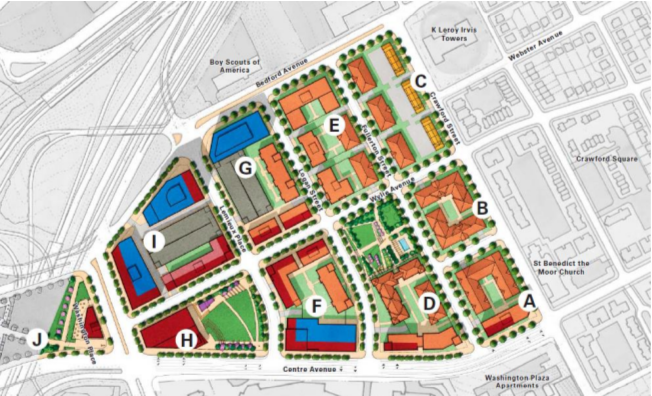
\includegraphics[width=0.5\linewidth]{mellonArena}
  \caption{Mellon Arena Project Site Plan View}
  \label{fig:mellonArena}
\end{subfigure}
~
\begin{subfigure}
  \centering
  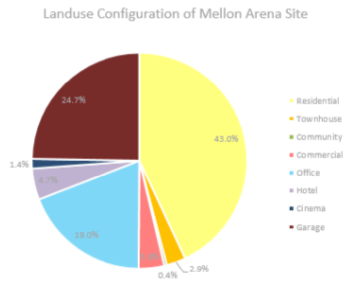
\includegraphics[width=0.3\linewidth]{mellonPie}
  \caption{Mellon Arena Site Land use Configuration}
  \label{fig:mellonPie}
\end{subfigure}
\end{figure}
The 16 building types in DOE commercial benchmark models do not
perfectly correspond to those in the Mellon Arena Site. In order to
adapt the topological pattern of the Mellon Arena Project, a mapping
(function) from building type of Mellon Arena Site to building type of
DOE models is created as follows:
\begin{table}[h!]
  \centering
  \begin{tabular}{c| c| c}
    \hline
    Mellon Arena Type &Probability &DOE Building Type\\
    \hline
    Hotel &50\%&Large Hotel\\
    \cline{2-3}
    &50\%&Small Hotel\\
    \hline
    Office &30\%&Large Office\\
    \cline{2-3}
    &30\%&Medium Office\\
    \cline{2-3}
    &30\%&Small Office\\
    \hline
    Residential &100\%&Midrise Appartment\\
    \cline{1-2}
    Townhouse &100\%&\\
    \hline
    Commercial &25\%&Full Service Restaurant\\
    \cline{2-3}
    $+$ Cinema $+$&25\%&Quick Service Restaurant\\
    \cline{2-3}
    Community &25\%&Super Market\\
    \cline{2-3}
    Center &25\%&Stand-alone Retail\\
    \hline
  \end{tabular}
  \caption{Mapping of Mellon Arena to Building Types of DOE benchmark model}
  \label{tab:typeMap}
\end{table}
The four major building types are residential, commercial, office and
hotel. Their topological pattern is represented in Figure
\ref{fig:mellonTop}. The conceptual model construction follows the
building type topological pattern and the urban density as the Mellon
Arena Project (\fref{fig:sitePlan})
\begin{figure}[h!]
  \centering
  \begin{subfigure}
  \centering
  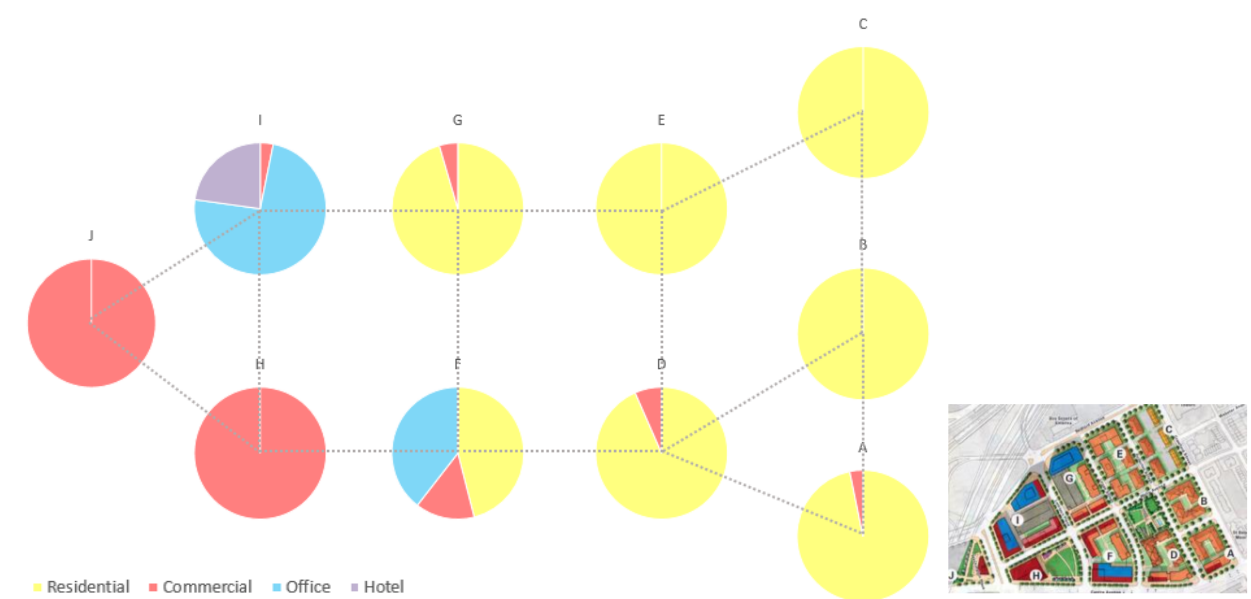
\includegraphics[width=0.7\linewidth]{mellonTop}
  \caption{Building Type Topological Pattern, Mellon Arena}
  \label{fig:mellonTop}
  \end{subfigure}
  ~
  \begin{subfigure}
  \centering
  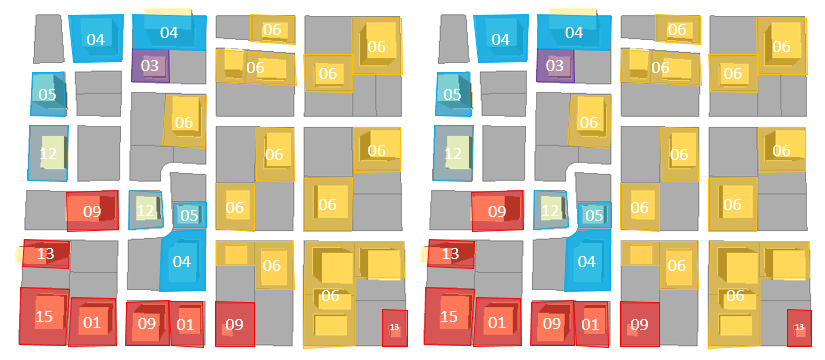
\includegraphics[width=0.7\linewidth]{sitePlan}
  \caption{Site Plan of Conceptual Model}
  \label{fig:sitePlan}
  \end{subfigure}
\end{figure}   

\subsection{Data Collection and Analysis}
\subsubsection{Simulation Data Analysis of the benchmark models}
The output of EnergyPlus simulation of 16 benchmark buildings are read
and processed with python script. This data loading and processing
module is used in both data analysis and the dynamic plot in the
interface design.

By analysing the simulation result of the Heating Energy (Gas) and the
Cooling Energy (electricity), we observed a large variation between
different building types.

Heating demand profile ranges

Hospital and Outpatient Health Care has a more spread out heating
demand (Gas) for all year round, this pattern is revealed in the
box plot graph. Comparing to these two building types, the other
benchmark buildings have a more concentrated demand pattern, with high
heat demand for winter and near-zero or zero heat demand over half of
the year (except for Large Hotel, Small Hotel and Midrise
Apartment). This indicates that these two building types could become
the major ``heat sink'' or anchor building to be connected to a
district system. In terms of peak demand, Large Office and Secondary
School has the highest peak heating demand, indicating the high heat .
\begin{figure}[h!]
  \centering
  \begin{subfigure}
  \centering
  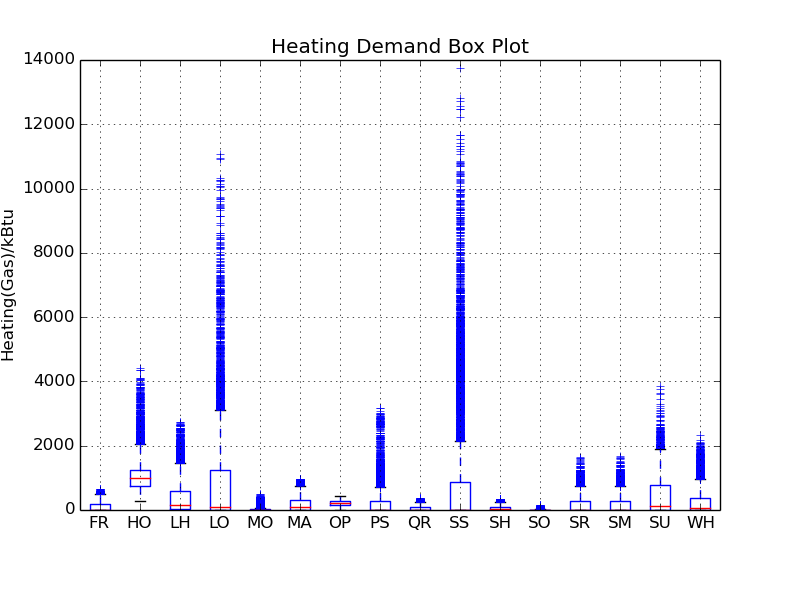
\includegraphics[width=0.7\linewidth]{heatBox}
  \caption{Heating Demand Box Plot}
  \label{fig:heatBox}
  \end{subfigure}%
  ~
  \begin{subfigure}
  \centering
  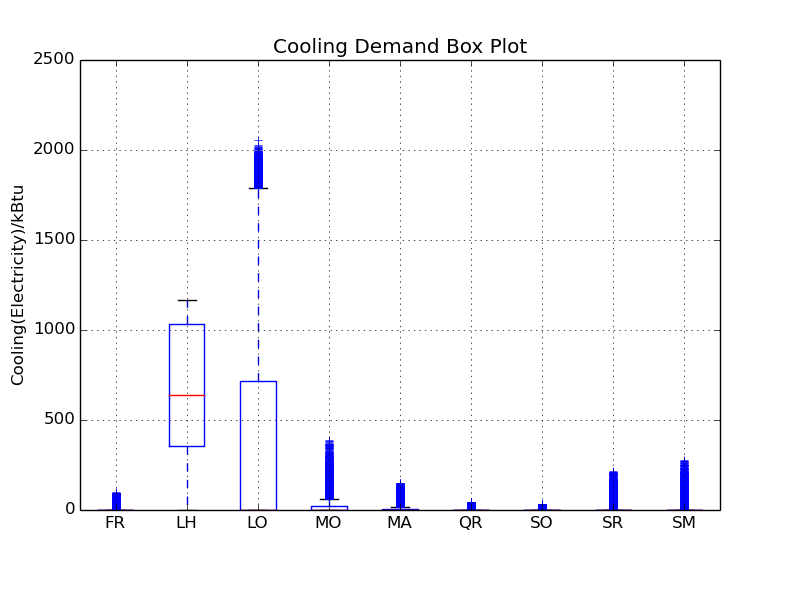
\includegraphics[width=0.7\linewidth]{coolBox}
  \caption{Cooling Demand Box Plot}
  \label{fig:coolBox}
  \end{subfigure}
\end{figure}   

\subsubsection{Potential Impact on system design or data visualization
  based on the analysis above}
The heating and 
\subsection{Temporal Data Aggregation}
      \begin{enumerate}[label*=\arabic*.]
      \item With CityEngine
      \item With ArcGIS (ArcScene)
      \item Comparison
      \end{enumerate}
\subsection{Data Classification and symbol/color design of a
        dynamic choropleth map}
    \begin{enumerate}[label*=\arabic*.]
    \item Review of General Approaches: see 3.3
    \item ``Critical Values'' or special cutoff values to be
      considered in the context of Community Energy Planning: need to
      look up (@@)
    \item Final choices of classification method and symbol/color
      scheme and the implementation
    \end{enumerate}

\newpage
\section{Interface Specification}
\subsection{Guidelines from interface design case study}
As is pointed out by Resch et al.\ , for 4D map visualization, one big
challenge lies in the cognitive aspect of human information
processing. Too much simultaneous stimuli might cause the degradation
in information retrieval and processing~\cite{Resch2014}. 

\subsection{User Definition}
We want to specify a user profile in order to best convey the
information with the Dynamic Energy Map.

The major category of user group for the Dynamic Map includes: 1)
policy makers, 2) urban planners with the interest in executing
community level energy strategys 3) researchers in energy related
fields 4) public groups or individuals that are involved or interested
in the decision making process of community energy planning.

The target user for the current interface design is restricted to
researchers in energy related fields. The assumption on this user
group about their skill level and background knowledge is that 1) they
have the basic ability to read and understand the layout of a map
environment and can associate it to the urban environment setting they
are associated with 2) they have the ability to correctly understand
moderately complicated map legend and data plot 3) they have the basic
understanding of related concept of building energy performance
attribute and the general implications of these attributes. The
assumptions about their intention is that they might have different
research interest and focus. These assumptions implies the interface
design should: 1) provide both qualitative and quantitative
information; 2) allow for some degree of user control over data
classification, legend selection and full control over time navigation

\subsection{Goal Function}
The goal function of the interface is defined as: revealing the
spatial-temporal heating / cooling demand variation of the conceptual
model by applying the Dynamic Energy Map on a conceptual urban
setting.

To assist district system design

\subsection{Specification of the Major Operation of the Interface}

The desired major operations for the target user include: 
\begin{itemize}
\item Map display and data plot
\item Navigation utilities that navigates through dynamic map and data
  plot
\item Provide default settings for choropleth map display
\end{itemize}

\subsubsection{Map display and data plot}
For researchers or planners: The desired map display should be a 2D
map with graduated symbol or color representing the heating or cooling
demand density, which is one of the major criteria of district system
sizing.  The map display should also be coupled with corresponding
data plot that providing the quantitative insight.

For general public: The desired map display should be a 3D map that
represents the actual building setup. Instead of using data plot, a
more intuitive bar chart of the aggregated demand could be more
helpful. The bivariate choropleth map legend should also be replaced
with two color ramps or even with only colors of extreme value. The
data classification method should also be chosen so that the peak
occurrence time is emphasized rather than the peak demand.

\subsubsection{Navigation utilities that navigates through dynamic map
  and data plot}
The ability to navigate through dynamic map images and dynamic data
plot, this is the basic function that differs the current work from a
static map. Some desired behavior of the slider includes:
\begin{itemize}
\item According to section \ref{anime}, the time has both linear and
  cyclic aspect. The time navigation utility should provide both
  ``linear'' time navigation and ``cyclic'' time navigation. This
  implies a global time navigation that can go through the time of
  year with the highest time resolution, and some navigation method
  with commonly used default time steps corresponding to the natural
  recurring pattern of the spatial-temporal data, energy usage profile
  for the current study.
\item Another desired feature is providing adjustable auto-play of the
  map animation. The reasoning behind this is the debatable level of
  user control in the study of Johnson and Nelson~\cite{Nelson1998},
  when they argue that allowing arbitrary time control might degrade
  the ability of animated map on conveying temporal pattern.
\item Exporting a time-animation with specified frame rate and with
  time-labels for each image and providing the choices to export the
  related dynamic plot together with the map to provide more
  quantitive insights. One of the draw back of the approaches of
  ArcGIS is its exported time-animation lacks proper time label and
  thus lost the quantative time information, making the resulted vedio
  only able to convey a rough intuition, severely degraded the ability
  of conveying the temporal spatial pattern.
\end{itemize}
\subsubsection{Provide default settings for choropleth map display}
Creating several default settings for choropleth map display,
i.e. provide choices for data classification and color mapping. For
the current implementation, the variables in display is the heating
and cooling energy consumption profile. The customization choices only
restrict to the two classification method: even or quantile
method. The color ramp is predefined to be a bivariate color ramp from
white to red and blue. For later stages, a desired behavior would be
to provide the full control of color settings.

\section{Interface Design}
\subsection {General Layout}
The interface for dynamic map display includes three major sections: a
series of sliders for controling images are on the left and the data
plot of energy profile of building sectors and aggregated demand are
on the right.

The main window on the top left is used for displaying the 2D dynamic
map of the conceptual model. The lower left of the window displays the
current time for the image and dynamic plot in display. The lower left
section contains a series of sliders for controling interactive
navigation of image and plot sequences. The right hand side of the
interface contains the dynamic data plot of the four major building
sectors: Hotel, Office, Residencial and Commercial buildings. The
lower right are the aggregated heating / cooling demand profile for
the whole site. The left column are the heating energy consumption in
natural gas and the right column are the cooling energy consumption in
electricity. On the lower right there are four buttons providing two
default forward and backward navigation, 1h and
24h. (\fref{fig:interface0720}).
\begin{figure}[h!]
  \centering
  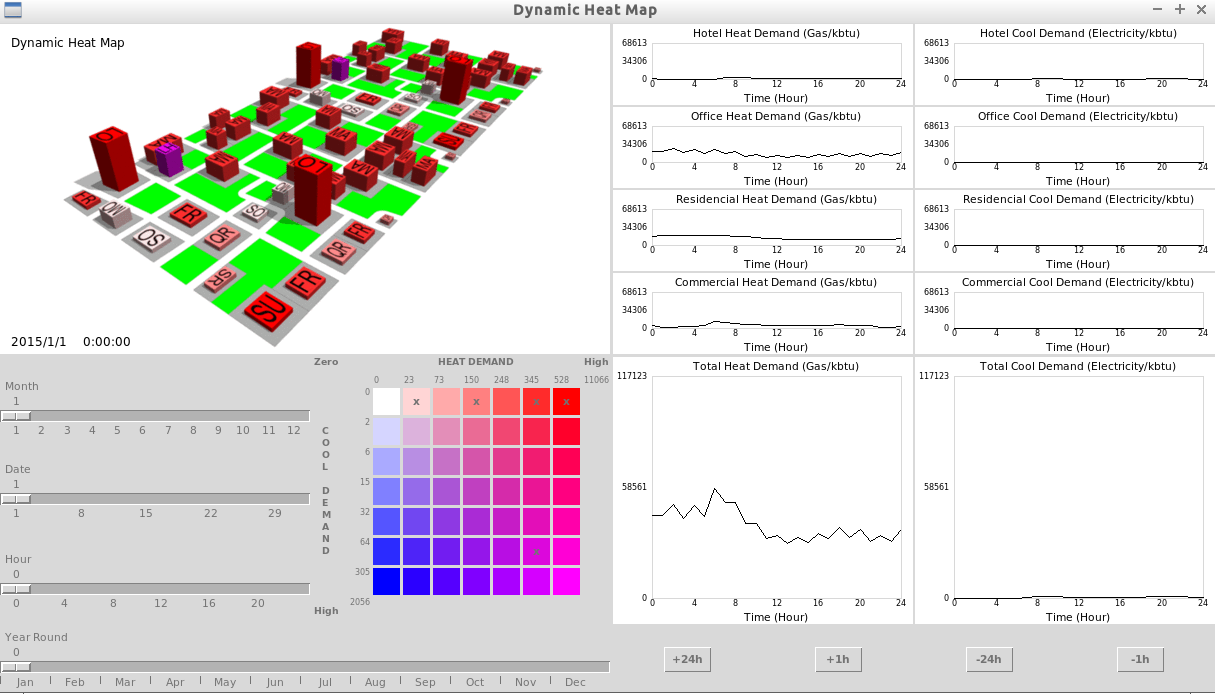
\includegraphics[width=0.7\linewidth]{interface0720}
  \caption{Dynamic Map Interface Layout}
  \label{fig:interface0720}
\end{figure}

Between the aggregated heat demand and the sliders, there is a
choropleth legend. According to section \ref{anime}, the comparison of
the map and the legend becomes tricky for dynamic maps. In order to
assist this task, tick marks of ``x'' are added to the legend to
indicate the color appeared in the map \fref{fig:legend}.
\begin{figure}[h!]
  \centering
  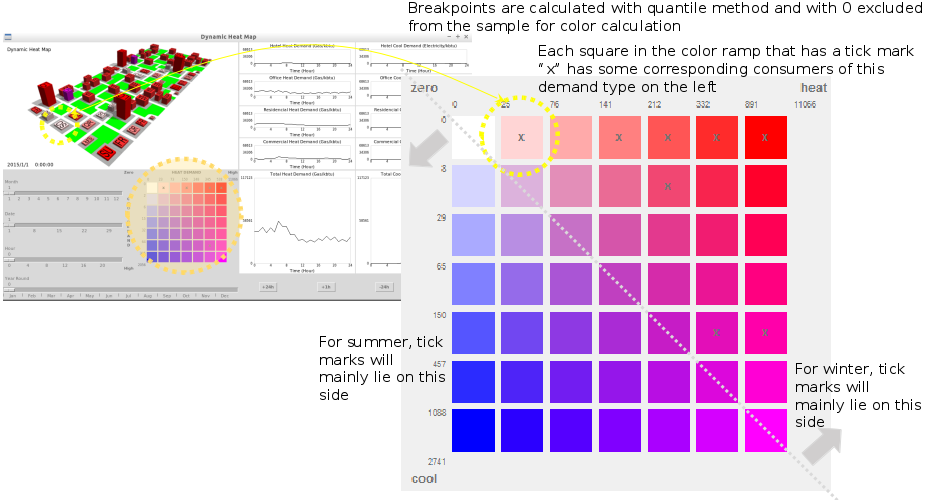
\includegraphics[width=0.7\linewidth]{legend}
  \caption{Bivariate Color Legend with Tick Mark Indicators}
  \label{fig:legend}
\end{figure}
\subsection {Navigation Function}
The navigation function is achieved with the four slider and the four
buttons above the sliders on the lower left of the window. The top
slider labeled with ``Year round'' has a range of 0 to 8760 (not
inclusive). the change of 1 in the slider position corresponds to the
change of 1 hour in time, which results in the display of the image of
the next or previous hour in time. The slider labeled with ``month''
has a range of 1 to 12, which corresponds to the 12 months in year,
the change of the month slider results the jump of 1 month forward or
backward in time. This function is intended to provide easy comparison
of montyly variation of the energy consumption behavior. Similarly,
the change of the ``date'' and ``hour'' slider corresponds to the time
change of one day or one hour respectively. The four buttons provides
a separate control intended to provide micro level adjustment of time.

\subsection {Dynamic Plot}
The input images to the main window is generated from the CityEngine
model. The graph is ploted by reading in simulation data from
EnergyPlus. The starting point (left end) of the plot corresponds to
the position indicated by the slider. 
\subsection {Implementation tools and strategy}
The softwares or platform involved in the project include EnergyPlus
for building simulation, CityEngine for 3D modeling and image
generation, Python 2.7 for interface design. The interface is written
in Python2.7 with standard Tkinter graphic package including the data
plot section.
\begin{comment}
\item Conclusion
  \begin{enumerate}[label*=\arabic*.]
  \item Summary of the current approach in implementing the dynamic
    Energy Map
  \item Limitations of the current implementation
    \begin{enumerate}[label*=\arabic*.]
    \item Simplified building simulation assumption about urban
      environment
    \item Lack of user choices for the stand-alone user interface as a
      result of its dependence on existing modeling softwares
    \end{enumerate}
  \item Future Expansion of the project
    \begin{enumerate}[label*=\arabic*.]
    \item Adding information of the supply side: residual energy,
      sustainable energy
    \item Providing different interfaces for different user population
    \item 2D and 3D compatible \\The reason for providing 2D map
      together with 3D map is that 2D maps have the following good
      properties:
      \begin{enumerate}[label*=\arabic*.]
      \item Better for region selection and spatial navigation than 3D
        map
      \item Better for conveying spatial relationship that does not
        involve height induced variation
      \item For larger scale display of city, state or nationwide, 3D
        building geometries becomes less significant in providing the
        urban environment context
      \end{enumerate}
    \item Creating an on-line tool for better information share
      \begin{enumerate}[label*=\arabic*.]
      \item Potential techniques: see 2.4
      \end{enumerate}
    \end{enumerate}
  \end{enumerate}
\item Acknowledgments
\end{enumerate}
\end{comment}
\newpage
\bibliographystyle{plain}
\bibliography{myCitation}
\end{document}